%\begin{savequote}[8cm]
%\textlatin{Cor animalium, fundamentum e\longs t vitæ, princeps omnium, Microco\longs mi Sol, a quo omnis vegetatio dependet, vigor omnis \& robur emanat.}

%The heart of animals is the foundation of their life, the sovereign of everything within them, the sun of their microcosm, that upon which all growth depends, from which all power proceeds.
  %\qauthor{--- William Harvey \cite{harvey_exercitatio_1628}}
%\end{savequote}

\chapter{The polycube codebase}
\label{ch:appendix_polycubes}

\minitoc

The code used for polycube assembly can be found at \url{https://github.com/akodiat/polycubes}. This code repository contains both the stochastic assembly code and the SAT solver code, as detailed in the sections below.

\section{Stochastic assembly code}
The polycube assembly model was implemented in both C++ and JavaScript. The C++ implementation enables the fast command--line evaluation of input rules required for the sampling performed in Chapter~\ref{ch:polycubes1}. Meanwhile, the JavaScript implementation makes it possible to assemble and visualise polycubes in a web browser, which was useful for both model validation and for public outreach activities.

In order to speedup sampling, the c++ binary can be called multiple times in parallel and merged with the merge python script. For the results covered in Chapter~\ref{ch:polycubes1}, the sampling was done on 100 concurrent nodes and merged.

The largest sampling done, the polyomino reference with 1e9 samples (described in Section~\ref{sec:refcalc}), took a total of 72 hours, 57 minutes, and 58 seconds to sample with 100 copies each performing 1e7 samples in parallel on 2.6 GHz CPUs. The merging script then took another 197 hours, 40 minutes, and 24 seconds to run, but it clearly saved a significant amount of time compared to running a single sampling for 100 times longer (which would take almost 7300 hours or 304 days). 

Finally the analysis script took another 301 hours, 44 minutes, and 17 seconds to run on the same hardware.

%took 359 hours, 9 minutes, and 44 seconds

\subsection{C++}
The stochastic assembly C++ code is found in the \texttt{cpp} directory. The Eigen and HDF5 libraries are required to compile the c++ binary. The python binding requires Eigen and the pybind library.

Install dependencies:
\begin{lstlisting}[language=bash]
  conda install -c conda-forge pybind11 eigen

  wget https://www.hdfql.com/releases/2.3.0/HDFql-2.3.0_Linux64_GCC-4.9.zip
  unzip HDFql-2.3.0_Linux64_GCC-4.9.zip
  mv hdfql-2.3.0 ~
\end{lstlisting}

The cmake specification at \texttt{cpp/src/CMakeLists.txt} is configured to search for HDFql at the path \texttt{\textasciitilde/hdfql-2.3.0}, so make sure to update the file if you install another version of HDFql or if it is installed at another path.

Build the polycube binary with cmake:
\begin{lstlisting}[language=bash]
  mkdir build && cd build
  cmake -DCMAKE_C_COMPILER=gcc -DCMAKE_CXX_COMPILER=g++ ..
  make
\end{lstlisting}

You should find the binary in the root of this directory (cpp)

Run ./polycubes --help for more info

\subsection{Python binding and analysis}
The C++ binary is used to sample the input rule space, as done in Chapter~\ref{ch:polycubes1}. However, to evaluate individual rules and access the stochastic assembly model through python, you can compile a pybind11 (\url{https://github.com/pybind/pybind11}) library that can be imported into python. There are build scripts and examples for both the python analysis scripts and the SAT solver code:

\begin{lstlisting}[language=bash]
  cd py
  bash build_pybind.sh
\end{lstlisting}

\begin{lstlisting}[language=bash]
  cd solve/py
  bash build_polycube_pybind.sh
\end{lstlisting}

This will generate a shared module \texttt{libpolycubes.so}

\begin{lstlisting}[language=python]
  import libpolycubes as pl
  pl.getCoords("040087000000")
\end{lstlisting}

The \texttt{py} directory contains a set of analysis scripts to interpret the results of the C++ binary output.

\subsection{JavaScript}
The JavaScript assembler is found in the \texttt{js} directory, with HTML files in the root of the repository. To run, you can either start a local webserver with the repository content or open the \texttt{index.html} file directly. You can also access the GitHub site at \url{https://akodiat.github.io/polycubes}.

The 3D visualisation is done with the help of the Three.js library (\url{https://threejs.org/}).

Polycube rules formatted as either decimal or hexadecimal strings (Section~\ref{sec:string_repr}) can be supplied to the assembler as URL arguments, for example: \url{akodiat.github.io/polycubes?decRule=|2:2|1:3||-3:0|_-1:1|-2:3||||_||||3:1|} and \url{akodiat.github.io/polycubes?rule=000a07008c00858b00000000000000000d00}.

\subsubsection{Patchy sphere preview}

Use the following script to generate patchy sphere preview images
\begin{lstlisting}[language=JavaScript]
  // Change cubes to spheres
  system.changeToSpheres()

  // Position camera (to get the same view angle)
  camera.position.copy(new THREE.Vector3(4,4,6).add(system.centerOfMass))
  camera.lookAt(system.centerOfMass)
  render()

  // Save image
  saveCanvasImage()
\end{lstlisting}

By default, the colours of species and patches only vary in hue. They can be made more diverse by also varying their saturation and luminosity:
\begin{lstlisting}[language=JavaScript]
system.particleMaterials.forEach(m=>{m.color.offsetHSL(0, 0.5*(Math.random()-0.5), 0.5*(Math.random()-0.5))})
system.colorMaterials.forEach(m=>{m.color.offsetHSL(0, 0.5*(Math.random()-0.5), 0.5*(Math.random()-0.5))})
\end{lstlisting}


\section{Polycube solver}

The polycube SAT solver code is found in the \texttt{solve} directory. As for the stochastic assembly code, the SAT solver has multiple implementation. The main implementation is done in Python and can be used for production runs. The other implementation is in JavaScript and is used to draw shape specifications and to solve smaller shapes.

\subsection{Python}

To use the python solver, you need to install the python-sat library:

\begin{lstlisting}[language=bash]
  python -m pip install python-sat[pblib,aiger]
\end{lstlisting}

To verify that the solver output assembles correctly, you also need to compile the polycube python binding:

\begin{lstlisting}[language=bash]
  cd solve/py
  bash build_polycube_pybind.sh
\end{lstlisting}

Finally, to solve a shape for a given number of species and colours, you call the \texttt{solve.py} script with the desired parameters:

\begin{lstlisting}[language=bash]
  python solve.py ../shapes/[shape].json [nSpecies] [nColors]
\end{lstlisting}

There are also ``multi--solve'' scripts to automatically create jobs solving all possible combinations of species and colour counts.

As an example of custom scripting, it is also possible to extract the CNF clauses to a file:

\begin{lstlisting}[language=python]
  import utils
  import json
  from polycubeSolver import polysat

  def saveClauses(nCubeTypes, nColors, solveSpecPath):
      with open(solveSpecPath, "r") as f:
          data = f.read()
      solveSpec = json.loads(data)

      mysat = polysat(
          solveSpec["bindings"],
          nCubeTypes,
          nColors,
          solveSpec["nDim"],
          solveSpec["torsion"]
      )

      name = solveSpecPath.split("/")[-1].split(".")[0]
      outPath = "{}t_{}c_{}.cnf".format(
          nCubeTypes, nColors, name
      )
      mysat.dump_cnf_to_file(outPath)

      print("Saved to {}".format(outPath))

  saveClauses(6, 9, "../shapes/scaling/cube4.json")
\end{lstlisting}

\subsection{JavaScript}
 The JavaScript implementation of the polycube solver is found in the \texttt{solve/js} directory, with the  HTML index file at \texttt{solve/index.html} directory. To use, you can either start a local webserver with the complete repository content and navigate to \url{http://localhost:8080/solve/index.html}, or access the GitHub site at \url{https://akodiat.github.io/polycubes/solve}.

 The web app provides an interface where you can interactively draw polycube shapes and save them as JSON shapes for the Polycube SAT solver. You can also use the console commands \texttt{drawFromCoords}, \texttt{drawSolidBlock}, and \texttt{drawSolidCube} to create shapes.

 You can also click a button to attempt to solve the shape within the browser. This is, however, usually only feasible for small shapes using SAT, so a substitution simplifier is also employed to work towards a minimal solution by substituting similar species in the fully addressable solution.


\chapter{Patchy particle model}
\label{ch:appendix_patchy}
As described in Section~\ref{sec:patchy_particles}, the patchy particle model is used is a derivative of the oxDNA patchy particle model used by Romano et al.\ \cite{rovigatti2015comparison}, modified to include torsional interactions to account for the polycube requirement of patch orientation alignment.

In the model, each particle is represented by a sphere covered by up to 6 patches at distance $R = 0.5$ distance units (d.u.) from the sphere's centre. The positions of the patches correspond to the three--dimensional Von Neumann neighbourhood around the origin:
$
 \mathbf{p}_1 = R \left( 0,1,0\right),\, \mathbf{p}_2 = R \left( 0,-1,0 \right),\,   %\\
 \mathbf{p}_3 = R \left( 0,0,1 \right),\, \mathbf{p}_4 = R \left(  0, 0, -1 \right),\, % \\
 \mathbf{p}_5 = R \left( 1,0,0 \right),\, \mathbf{p}_6 = R \left( -1, 0, 0 \right),
$
Each patch is additionally assigned an orientation $\mathbf{o}$, which is equal to
$\pm \mathbf{e}_1, \pm \mathbf{e}_2$, or $\pm \mathbf{e}_3$, which are the base vectors (or their negatives) of the orthonormal base of the particle. The orientation  $\mathbf{o}_a$ assigned to each patch $a$ satisfies $\mathbf{p}_a \cdot \mathbf{o}_a = 0$.

\begin{figure}[h]
\centering
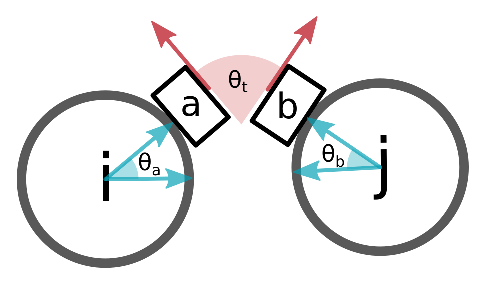
\includegraphics[width=0.8\linewidth]{figures/pp.eps}
\caption{Schematic of the patchy particle alignment angles. Note that, while the figure is drawn in 2D, the particles and vectors are in fact three--dimensional and are not restricted to the depicted plane. The angle \(\theta_a\) is measured between the vectors \(\mathbf{\hat{r}_{ij}}\) (pointing from particle \(i\) to particle \(j\)) and \(\mathbf{\hat{p}_a}\) (pointing from from particle \(i\) to its patch \(a\).  \(\theta_b\). Likewise, the angle \(\theta_b\) is measured between the vectors \(-\mathbf{\hat{r}_{ij}}\) (pointing from particle \(j\) to particle \(i\)) and \(\mathbf{\hat{p}_b}\) (pointing from from particle \(j\) to its patch \(n\). Finally the angle \(\theta_t\) is measured between the orientation vectors of the two patches, \(\mathbf{o}_{a}\) and \(\mathbf{o}_{b}\), which are always orthogonal to \(\mathbf{\hat{p}_a}\) and \(\mathbf{\hat{p}_b}\) respectively.
}
\label{fig:pp}
\end{figure}

We model the interaction between patches using point--like patch interaction, where the interaction between two patches $a$ and $b$ on two distinct particles $i$ and $j$ is given by the following interaction potential:
\begin{equation}
V_{\rm patch}(\mathbf{r}_{ij},\mathbf{\Omega}_{ij}) = \delta_{ab} V_{\rm pdist}(r_p) V_{\rm angle}(\theta_a, \theta_b, \theta_t)\,, 
\end{equation}
 where $\delta_{ab}$ is 1 if colours assigned to patch $a$ and $b$ are compatible and 0 otherwise. The patch potential consists of two components: potential $V_{\rm pdist}$ that only depends on distance between the two patches $r_{ab}$, and $V_{\rm angle}(\theta_a, \theta_b, \theta_t)$ which depends on the mutual orientation $\mathbf{\Omega}_{ij}$ of the two particles as given by angles that are calculated as follows:
\begin{equation}
\cos \theta_a =  \mathbf{\hat{r}}_{ij} \cdot \mathbf{\hat{p}}_a, \quad \cos \theta_b =  \mathbf{-\hat{r}}_{ij} \cdot \mathbf{\hat{p}}_b, \quad 
\cos \theta_t =  \mathbf{o}_{a} \cdot \mathbf{o}_b\,,
\end{equation}
where the above vectors are normalised to 1, as indicated by the hat symbol. As seen in Figure~\ref{fig:pp}, angles $\theta_a$ and $\theta_b$ correspond to the angle between the normalised vector between the centres of mass of patchy particle $i$ and $j$ and the normalised vector pointing to patch $a$ or $b$ respectively. Angle $\theta_t$ corresponds to the angle between the orientations associated with the respective patches. The interaction potential is 
\begin{equation}
    V_{\rm angle}(\theta_a, \theta_b, \theta_t) = V_{\rm angmod}(\theta_a) V_{\rm agmod}(\theta_b)
    V_{\rm agmod}(\theta_t)\,,
\end{equation}
where $V_{\rm agmod}$ is angular modulation function defined to be equal to one if the angle $\theta$ equals to the desired angle $\theta_0$ (which are set to $0$, requiring perfect alignment of the respective vectors), and parameters $a$ and  $\Delta$ then define the width of the potential.
\begin{equation}
V_{\rm angmod}(\theta) = \begin{cases}
	V_{\rm mod}(\theta, a, \theta_0)  & \text{if $ \theta_0 - \Delta < \theta < \theta_0 + \Delta  $},\\
	V_{\rm smooth} (\theta, b, \theta_0 - \Delta_c) & \text{if $\theta_0 - \Delta_c < \theta < \theta_0-\Delta $},\\
	V_{\rm smooth} (\theta, b, \theta_0 + \Delta_c) & \text{if $\theta_0 + \Delta < \theta < \theta_0+\Delta_c$},\\
	0 & \text{otherwise}.
	\end{cases} \,,
\end{equation}
where the additional parameters $b$ and $\Delta_c$ are set so that the piece--wise function $V_{\rm angmod}(\theta)$ is differentiable (See Figure~\ref{fig:narrow_types}). The potentials used in the definition are 
\begin{equation}
\label{eq:smooth}
V_{\rm smooth} (x, b, x_c) = b(x_c - x)^2
\end{equation}
and
\begin{equation}
V_{\rm mod} (\theta, a, \theta_0) = 1 - a (\theta-\theta_0)^2\,.
\end{equation}

Unless otherwise specified, the default narrow type 0 was used, with 
$a = 0.46$ and $\Delta = 0.7$ for $V_{\rm angmod}$ as seen in Figure~\ref{fig:narrow_types}.

\begin{figure}[h]
%\centering
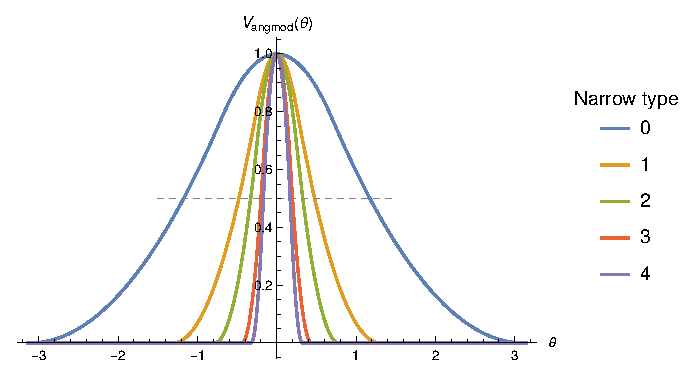
\includegraphics[width=\linewidth]{figures/patchysim/nts.eps}
\begin{tabular}{|c|l||l|l|l|l|l|}
    \hline
    nt & width & \(\theta_0\) & \(\Delta\) & \(\Delta_c\) & \(a\) & \(b\) \\ [0.5ex] 
    \hline\hline
    0 & 2.345750 & 0 & 0.7 & 3.105590 & 0.46 & 0.133855 \\
    1 & 0.954736 & 0 & 0.2555 & 1.304631 & 3 & 0.730604 \\
    2 & 0.656996 & 0 & 0.2555 & 0.782779 & 5 & 2.42282 \\
    3 & 0.396613 & 0 & 0.17555 & 0.438183 & 13 & 8.689492 \\
    4 & 0.336622 & 0 & 0.17555 & 0.322741 & 17.65 & 21.0506 \\
    \hline
\end{tabular}
\caption{Patchy particle narrow types, causing patches of different widths. The table shows the constants used for each narrow type, with the plot showing the different angular modulation potentials as a function of angle in radians. The width is measured between the two points intersecting the dashed line, where \(V_{\text{angmod}}=\frac{1}{2}\). The default narrow type \(0\) is the least narrow. }
\label{fig:narrow_types}
\end{figure}

The additional distance--modulation term in the potential between a pair of patches on two distinct particles is 
\begin{equation}
    \label{eq_patch}
    V_{\rm pdist}(r_p) =  \begin{cases} 
                          %-1.001 \delta_{ij} e^{- \left( \frac{r_p}{\alpha} \right)^{10}} - C & \text{if $r_p \leq r_{\rm pmax}  $}\\
                          -1.001  \exp{\left[- \left( \frac{r_p}{\alpha} \right)^{10}\right]} + C & \text{if $r_p \leq r_{\rm pmax}  $} \\
                          0 & \text{otherwise}
                        \end{cases}
    %e^{ -\left( \frac{r - \delta}{\sigma} \right)^2}
    \,,
\end{equation}
where $r_p$ is the distances between a pair of patches, and $\alpha = 0.12\, {\rm d.u.}$ sets the patch width. The constant $C$ is set so that $V_{\rm patch}(r_{\rm pmax}) = 0$ for $r_{\rm pmax} = 0.18\, \rm{d.u.}$. The patchy particles further interact through excluded volume interactions ensuring that two particles do not overlap:
\begin{equation}
    f_{\rm exc}(r,\epsilon,\sigma,r^{\star}) = \begin{cases}
	V_{\rm LJ}(r, \epsilon, \sigma) & \text{if $r < r^{\star} $},\\
	\epsilon V_{\rm smooth} (r, b, r^c) & \text{if $r^{\star} < r < r^c$},\\
	0 & \text{otherwise}.
	\end{cases}
  \,,
\end{equation}
where $r$ is the distance between the centers of mass of the patchy particles, and $\sigma$ is set to $2R = 1.0$ distance units, twice the desired radius of the patchy particle.
The repulsive potential is a piecewise function consisting of the Lennard--Jones potential function:
\begin{equation} 
V_{\rm LJ}(r,  \sigma) = 8 \left[ \left(\frac{\sigma}{r}\right) ^{12} - \left(\frac{\sigma}{r}\right) ^{6} \right].
\end{equation}
that is truncated using a quadratic smoothing function from \eqref{eq:smooth}, with $b$ and $x_c$ set so that the potential is a differentiable function that is equal to $0$ after a specified cutoff distance $r^c = 0.8$.  

The patchy particle system was simulated using rigid--body Molecular Dynamics with an uring the simulation, each patch was only able to bind to one other patch at the time, and if the binding energy between a pair of patches, as given by Eq.~\eqref{eq_patch}, is smaller than 0, none of the patches can bind to any other patch until their pair interaction potential is again 0.


\section{Patchy particle code}

The modified version of oxDNA used to simulate torsional patchy particles can be found at \url{https://github.com/Akodiat/oxDNA_torsion}. To download and combile, run:

\begin{lstlisting}[language=bash]
  git clone https://github.com/Akodiat/oxDNA_torsion.git
  cd oxDNA_torsion
  mkdir build
  cd build
  cmake ..
  make -j4
  make romano
\end{lstlisting}

Simulation files for a given polycube shape can then be generated through the web console at \url{https://akodiat.github.io/polycubes}, by running:

\begin{lstlisting}[language=JavaScript]
  getPatchySimFiles(
    "070000070500868700000000", // Rule string
    1, // Number of assemblies
    "cube", // Name
    "/users/joakim/repo/oxDNA_torsion", // Path to oxDNA directory
    [.01,.02,.03,.04,.05,.06,.07,.08,.09,.1], // Temperature range
    0.1 // Density (used to generate configuration when the number
    // of assemblies is more than one)
  )
\end{lstlisting}

If the number of assemblies is one, a configuration file will be generated specifying the assembled shape. Else, the \texttt{generateConf.sh} script can be used to generate a random configuration with the provided density.


\chapter{The oxView codebase}

The code for oxView can be found at \url{https://github.com/sulcgroup/oxdna-viewer}. It is written in TypeScript and compiled into JavaScript. The 3D visualisation is done with the help of the Three.js library (\url{https://threejs.org/}), while the graphical user interface uses the Metro 4 library (\url{https://metroui.org.ua/}). 

If you make any changes, you need both TypeScript (\url{https://www.typescriptlang.org/}) and Node.js (\url{https://nodejs.org/}) installed to compile. Typing \verb|npm install| in the source directory should install all required node modules. Then type \verb|tsc| to compile the typescript into javascript. 

More detailed documentation can be found in the README.md file in the repository: \url{https://github.com/sulcgroup/oxdna-viewer/blob/master/README.md}

\minitoc

